\documentclass[conference]{IEEEtran}
\IEEEoverridecommandlockouts
% The preceding line is only needed to identify funding in the first footnote. If that is unneeded, please comment it out.
\usepackage{cite}
%\usepackage{caption}
%\usepackage{subcaption}
\usepackage{tikz}
\usetikzlibrary{shapes.geometric,arrows, positioning, fit, calc}
\usepackage{amsmath,amssymb,amsfonts}
%\usepackage{algorithmic}
%\usepackage{algorithm}
%\usepackage{graphicx}
%\usepackage{xcolor}
%\usepackage{epsfig}
%\usepackage{mathptmx}
%\usepackage{textcomp}
%\usepackage{mathtools}
%\usepackage{lipsum}
%\usepackage{gensymb}
\tikzstyle{computing} = [draw, rectangle, fill=white!50, rounded corners, node distance=3em, minimum height=3em]

\tikzstyle{io} = [rectangle, draw, trapezium right angle=110, rounded corners,
                  fill=red!20, node distance=5em, minimum height=2.9em]

\tikzstyle{calculate} = [diamond, draw, trapezium right angle=110, rounded corners,
                  fill=green!20, node distance=1.9cm, minimum height=2.9em]

\tikzstyle{hardware} = [rectangle, draw, trapezium right angle=110, rounded corners,
                  fill=blue!20, node distance=1.9cm, minimum height=2.9em]

\tikzstyle{external} = [rectangle, draw, trapezium right angle=110, rounded corners,
                  fill=gray!20, node distance=1.9cm, minimum height=2.9em]
\tikzstyle{line} = [draw, -latex']

\tikzstyle{function} = [rectangle, draw, fill=green!20, node distance=1.9cm, minimum height=2.9em]

\def\BibTeX{{\rm B\kern-.05em{\sc i\kern-.025em b}\kern-.08em
    T\kern-.1667em\lower.7ex\hbox{E}\kern-.125emX}}

    \title{Project Report*\\
    {\footnotesize \textsuperscript{*}As a fulfilment to the course: "Project course name",
     D7039E \& E7032E. Lecturer: Jan van Deventer.}
    %%\thanks{Identify applicable funding agency here. If none, delete this.}
    }
    
    \author{\IEEEauthorblockN{Martin Blaszczyk, Edward Cedegård, Niklas Dahlquist, Edward Källstedt, Albin Martinsson, Måns Norell}
    \IEEEauthorblockA{\textit{Computer Science, Electrical and Space Engineering Dept.} \\
    \textit{Lule{\aa} University of Technology}\\
    Lule\aa, Sweden \\
    \{marbla-6, edwced-4, nikdah-6, edwkll-7, mnsnor-5, albmar-6\}@student.ltu.se}
    }
\date{\today}

\begin{document}
\maketitle
\begin{abstract}
\end{abstract}

\section{Introduction}
\subsection{Background and Motivation}
% Short Arrowhead introduction
Arrowhead is an initiative from Luleå University of Technology to create a unifying framework which can enable embedded devices to intergrate and interoperate services in an open-network environment. This framework and its approach will strongly conribute to the reduction of design and engineering efforts in the industry. 

% Why project course?
As part of the Engineering Project course for Master's students in Computer Science, Control and Electrical Engineering at Luleå University of Technology the goal is to implement and demonstrate how the Arrowhead Framework can be used in a factory setting using autonomous ground robots. This project report aims to give an overview of the thought process, workflows and results of the project.

The proposed solution is a robot which by implementing machine vision algorithms can navigate the factory floor while also being able to pick up objects using it's arm and gripper. It utilizes the Arrowhead framework to integrate with the other parts of the model factory. 

\subsection{Contributions}
Our proposed solution is an example of how the Arrowhead framework is utilized in a scaled factory setting together with a ground robot. The design is small and modular making it easy for future improvements and easy evaluation of the Arrowhead framework alongside third-party open-source solutions. Secondly we propose a solution consisting of colored lines and QR-codes and how the robot can follow a path using a RGB-camera instead of the conventional sensors such as IR-sensors. With this camera solution the possibilities of navigating the factory floor increase compared to the basic conventional following solutions. 
\section*{Structure}
The overall structure of the report...

\cite{ros}

\section{Arrowhead}
\section*{Arrowhead}
What is it?
\section*{Extras}
More in depth about the strucutre of the Arrowhead implementation. Flow diagrams etc. 

\section{Concept Design}
\section*{Mechanical structure}
The final design of the robot. Include CAD renderings etc. 
\section*{Electrical components}
Electrical components such as motors, MCUs etc. Why were they chosen

\section{Modeling}
\section*{Robotic arm}
\subsection*{Forward kinematics}
\subsection*{Inverse kinematics}


%%%%%%%%%%%%%%%%%%

\section*{Base}

 The motors will be connected to tracks on the robot and can therefore be modelled as two wheels connected with a rod, as seen in figure \ref{fig:base_math_model}.\\ 
This means that most of the mathematical modeling is very straight forward given that we can read the encoders from the motors. From the encoders we would be able to get both the length the robot has traveled and more importantly the individual speed each motor rotates with. The speed for the individual motor is of course given by: 

\begin{equation}
    v_m=\frac{2\pi r_{wheel}/N_{encoders}}{\Delta t}
    \label{eq:base_system_eq1}
\end{equation}

\noindent Where $N_{encoders}$ is the number of encoders on the motor, $r_{wheel}$ is the radius of the driving wheel and thickness of the track and $\Delta t$ is the time between the previous encoder reading and the most recent one. By doing this for both the left and right motor we can find how fast the robot is moving along the line by:

\begin{equation}
    \overline{v}= \frac{v_L+v_R}{2}(-\cos \theta \hat{i}+ \sin \theta \Hat{j})
\end{equation}

\noindent Where the $y$-axis parallel to the line. In a similar fashion to how we calculated the velocity of the robot, the rate of change of the angle can be calculated using:

\begin{equation}
    \Dot{\theta} = \frac{v_R-v_L}{2r_{base}}
    \label{eq:base_system_eq2}
\end{equation}

\noindent Where $r_{base}$ is the distance from the center of the base to the wheels. From this and figure \ref{fig:base_math_model} it's easy to see that the change of angle then becomes:

\begin{equation}
    \theta = sin^{-1}\left(\frac{V_L-V_R}{2r_{base}}t\right)
\end{equation}

\begin{figure}[H]
    \centering
    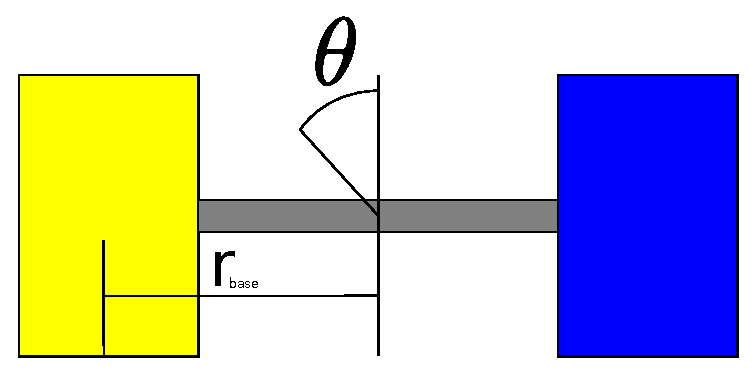
\includegraphics[width=0.7\textwidth]{base_math_model.eps}
    \caption{Modelling of the base as two wheels connected with a rod, where $\theta$ is the angle to the line}
    \label{fig:base_math_model}
\end{figure}

Given small angles \footnote{Which will be assumed because the robot will be operating on a grid with hard coded functions for turning at QR-codes}, we can therefore write this as:

\begin{equation}
    \theta = \frac{V_L-V_R}{2r_{base}}t
\end{equation}


\noindent Using equations \eqref{eq:base_system_eq1}-\eqref{eq:base_system_eq2} a system can be built for simulations in matlab, using rate of change and max/min value limiters for simulations of the motors physical restrictions.

%%%%%%%%%%%%%%%%%%%%%%%%%%%%%%%%%


\section*{Camera vision and calibration}
In this section it is outlined the theory behind the camera vision system. 
How points in a 3D-space are projected on a 2D-plane, calibration and distortion correction. 
\subsection*{Camera model}
\subsection*{Distortion}


\section{Machine Vision}
\section*{Line following}
\section*{QR-codes reading}
\section*{Deep learning?}

\section{Motion}
\section*{Robot arm}
\section*{Path planning}
preliminary stuff
\begin{itemize}
    \item Since the base use tracks, it can turn on a point. Therefor the turning radius will be the length from the center of the tracks, to the object furthest away from the center.
    \item The acceleration need to be slow enough to not tip the robot over, since it seems quite top heavy.
    \item The motors will need decoders for some of the control to work, if done the way they're planed
    \item The motors also need to be strong enough to move the robot, both with and without load.
\end{itemize}

\section{Experiment}
\section*{Prototype components}
Overview of what is being used in the evaluation
\section*{Movable base evauation}
\section*{Arm evaluation}
\section*{Gripping evaluation}
\section*{Sensor evaluation}
\section*{Machine vision evaluation}
The line following algorithm has generally worked well.
During testing the robot has been able to follow the lines and identify the QR codes.
The robot is able to travel between points in the grid in a sufficient manner.

%Limitation 1
A limitation of the line following algorithm is its sensitivity to noise.
Bad lighting conditions and a poorly calibrated color mask can negatively affect the ability to track the line reliably.
A possible future optimization to mitigate this effect would be to keep track of the center point of the line in the previous frame.
The image moment calculation could then be done in a smaller subsection of the horizontal slice around the previous center.
Currently, the algorithm uses the entire width of the frame to calculate the center point.
This leads to a heightened sensitivity to random noise in the outer parts of the frame.
If the general position of the line is already known only pixels close to this point should be considered, since the line will not move considerably between frames.

% Limitation 2
Also, another limitation is the fact that the machine vision system is dependent on sufficiently fast hardware.
Some lag will always be introduced while the current image is being processed.
If the hardware on which the system is run is slow this lag runs the risk of being alarmingly large.
This will result in the angle sent to the base controller being out of date.
However, when running on a Raspberry Pi 4 or the Nvidia Jetson Nano this delay is negligible.
This can also be tuned by changing the image resolution used to capture frames with the camera.
Preferably, the resolution should be low to increase performance but not so low that the ability to recognize QR codes is impaired.
During testing $360$ by $240$ was found to be a good middle ground between performance and image quality.
\section*{Arrowhead evaluation}

\section{Conclusions}
Conclusions of the robot and the course (?)





\section*{Conceptual design}

\newpage
\appendix
% !TeX root = ../main.tex

\section*{Martin Blaszczyk}
Martin is a 5th year Y-student with interest in Control och Mechatronics. 
In this course he'll take the role of the Project Leader where the main objectives
are to keep focus on the goal, hold meetings and an overall oversight of the project. 
As for the technical part the main interest will be in machine vision together with
Edward K. to use cameras or other sensors to localize external objects for the 
robot to grip, avoid or approach.

\section*{Edward Cedgård}

Master in  electronic systems and control engineering.
Edward's main task is to design the robotic arm and gripper mechanism together with Niklas. 
Tasks as deriving the kinematic equations, and implementation using forward and inverse kinematics.
Choise of motors, armdesign, communication with motors using serial communication. 

\section*{Niklas Dahlquist}
Niklas is studying his fifth year at the Engineering physics and electrical engineering student program.

His main focus will be to work with Edward Cedgård to evaluate the gripping mechanism and if necessary design new components and model the corresponding control system to be able to lift up and hold the target object.

\section*{Edward Källstedt}
Currently studying his fourth year in the Master Programme in Computer Science and Engineering.
A fan of making things secure, fast, scalable, and well-documented. Primarily interested in
low level software development. Will initially work on the machine vision implementation 
together with Martin. In addition to machine vision specifically this work will also consist
of robot localization and collision avoidance. As the project progresses he will take on more
general software problems that might arise. The first week will be spent researching different
computer vision technologies.


\section*{Albin Martinsson}
Albin is a 5th year computer science student specializing in industrial computersystem. 
In this project he will be focusing on the arrowhead integration and bein charge of the Github repository.  
This will entail connecting all the services toeach other and making sure they are authenticated and secure.  
Being in chargeof the git repository will entail merging pull requests and sorting out conflicts,
making sure that the version control part of this project runs smoothly.


\section*{Måns Norell}
Studying for a master in electronic systems and control engineering.
Måns main task is to design the base and line-following controller for moving the robot along a line. 
Tasks include designing the base, printing the specialized parts, simulating and testing the base.
Communication between controller, motor and camera will be worked on in collaboration with those in charge of these tasks. 


\section{Working together}
\section*{Project structure}
To keep the project going and have an organized structure the project is divided 
in different parts, or subprojects. Each group member is either alone or in group responsible for each part of the project which coincides with their interests. 
\begin{itemize}
    \item Arrowhead
    \item Machine vision and localization of external objects
    \item Gripping tool
    \item Movable base
\end{itemize}

\section*{Meetings}

Every week the group met on Mondays and Thursdays to catch up and support each other. This structure gave the students a great deal of responsibility to do work for each meeting while still maintaining a good structure of the project and encouraged discussions. 
The agenda of the monday meeting was:
\begin{itemize}
    \item Status of work done the previous week by each member
    \item Preparation for the seminar
    \begin{itemize}
        \item Discussion of the previous seminar meeting
        \item How the weeks work has been coinciding with the seminar feedback
        \item Questions to ask the teachers
        \item Questions to ask the other group
        \item Who does what during the seminar
    \end{itemize}
    \item Other
\end{itemize}
The Thursday meeting was to collect and reflect over the 
feedback from the teachers and the other group from the seminar. Also a status on the work planned to be done the following week was discussed so that each member had a good understanding of what the other members were doing. Those meetings had had the following agenda
\begin{itemize}
    \item What feedback did the teachers give
    \item What feedback did he other group give 
    \item Feedback to each other withing the group
    \item Work to be done the following week
    \item Other 
\end{itemize}

\subsection{Project planning}
The projects course started in August 2020 and continued until mid January 2020 with the project deadline in the middle of December. To keep a good structure and to synchronize all the parts of the project a plan was made, shown in Table \ref{tab:overall_time_plan}. This plan enabled the group to be flexible and maintain a good long-term structure of the project. Every month a more detailed time plan was prepared to facilitate the small changes, delays etc. 
\begin{frame}
    \subsection{Time plan}
    \frametitle{Overall timetable}
    \begin{table}
        \begin{tabular}{| l | c | c | c | c }
            
            Sep & Oct & Nov & Dec \\
            \hline \hline
            Concept generation & Evaluation & Evaluation &  \\ 
            \hline
            Theory & Prototyping & Evaluation & Finishing up \\
            \hline
            Simulation & Evaluation & Evaluation & \\
            \hline
            Prototyping & Final Design & Evaluation &  \\
            \hline
 
        \end{tabular}
    \end{table}    
\end{frame}

\begin{frame}
    
    \frametitle{Time plan for October}
    \begin{table}
        \begin{tabular}{l | c | c | c | c }
        Subproject & Week 1 & Week 2 & Week 3 & Week 4 \\
        \hline \hline
            Arrow & Working & Structure & Fusion & ...\\
            Base & CAD & Communication & ROS & Final\\
            Arm  & Assembly & Gripper & ROS & Final\\
            MV & Porting to NVIDIA & API & Evaluation & ...\\
        \end{tabular}
    \end{table}
\end{frame}



For the group members to what task were to be done, the built in function of Issues on the souce control platform Github\textregistered \ was utilized. A Milestone was created for each week and populated with issues. When an issue was finished it could simply be closed. If the issue was delayed it showed clearly in the Issue overview which tasks had to be prioritized. 

\subsection{Source control}
To keep track of the different software implementation the projects source control implements Git in one common repository \cite{repo}. The repository is where all source code and relevand 3D-files are located. This report is written in LaTeX with Git as source control. To make sure it's easy for all members to write their designated sections a workflow was designed to to minimiza merge conflicts while writing drafts as show in Fig. \ref{fig:git_workflow}. Without this flow the group members would experience merge conflicts after every push which would make it more complex and time consuming.

    \begin{figure}
        \begin{center}
\resizebox{6.0cm}{!}{

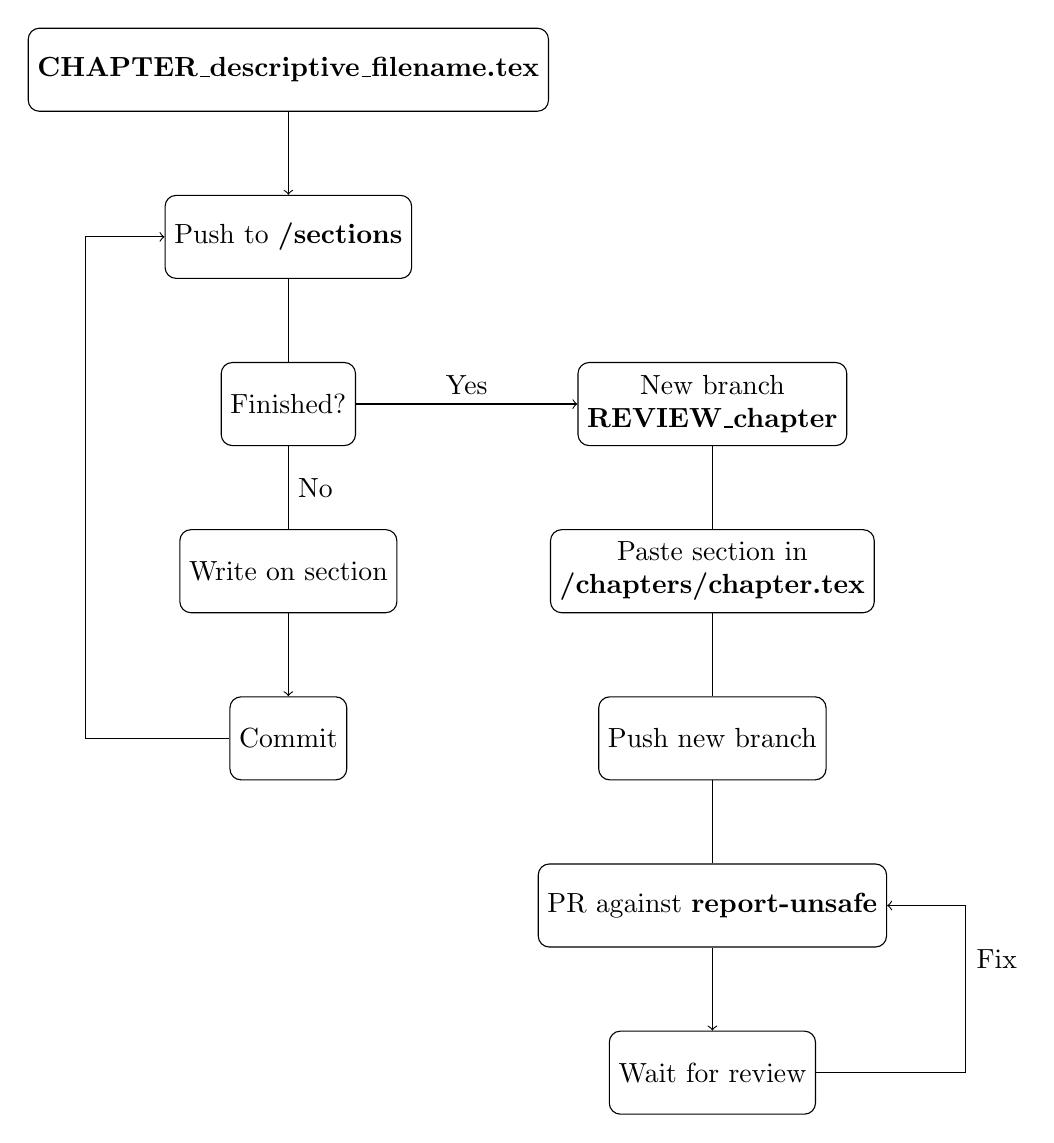
\begin{tikzpicture}
    [align=center, auto]
    \node [computing] (start) {\textbf{CHAPTER\_descriptive\_filename.tex}};
    \node [computing, below= of start] (push) {Push to \textbf{/sections}};
    \node [computing, below= of push] (finished) {Finished?};
    \node [computing, below= of finished] (write) {Write on section}; 
    \node [computing, below= of write] (commit) {Commit};

    \node [computing, right= of finished, xshift=5em] (branch) {New branch \\ \textbf{REVIEW\_chapter}};
    \node [computing, below= of branch] (paste) {Paste section in \\ \textbf{/chapters/chapter.tex}};
    \node [computing, below= of paste] (pushb) {Push new branch};
    \node [computing, below=of pushb] (PR) {PR against \textbf{report-unsafe}};
    \node [computing, below= of PR] (review) {Wait for review};
    
    



    \coordinate [left= of push] (lrpush);
    \coordinate [left= of write] (lrwrite);
    \coordinate [left= of commit] (lrcommit);
    \coordinate [left= of finished] (lrfinished);
    \coordinate [right= of PR] (crPR);
    \coordinate [below= of crPR] (crreview);
    



    \draw [->] (commit) -- (lrcommit) -| (lrpush) -- (push);

    \draw [->] (start) -- (push);

    \draw [->] (push) -- (finished) -- node[midway, fill=white] {No} (write) -- (commit);

    \draw [->] (finished) -- node[midway, fill=white] {Yes} (branch);

    \draw [->] (branch) -- (paste) -- (pushb) -- (PR)  -- (review);

    \draw [->] (review) -| (crreview) -- node[midway, xshift=2.2em, yshift=-0.5em, fill=white] {Fix} (crPR) -- (PR);
    
    
\end{tikzpicture}
}
\end{center}
\caption{Report writing flowchart}
\label{fig:git_workflow}
\end{figure}














\bibliographystyle{IEEEtran}

\bibliography{bibliography.bib}

\end{document}





